\chapter{Testy nowej wersji oprogramowania}
\label{cha:test}
Niniejszy rozdział zawiera opis testów systemu GGSS przeprowadzonych na koniec trwania prac związanych z oprogramowaniem systemu GGSS. Celem testów była weryfikacja poprawności działania czterach konfiguracji programu \textit{ggssrunner}: wersja deweloperska (\textit{debug}) ze statycznie linkowaną biblioteką \textit{Boost}, wersja deweloperska z dynamicznie linkowaną biblioteką \textit{Boost} oraz analogiczne wersje produkcyjne (\textit{release}). Z uwagi na powtarzalny charakter procesu testowania zaprezentowany zostanie jedynie przebieg testów dla wersji \textbf{deweloperskiej ze statycznie linkowaną biblioteką Boost}. 

\section{Przebieg testu}
Ze względu na fakt, że środowisko w którym osadzony jest program \textit{ggssrunner} jest ciągle monitorowane, pierwszym krokiem było umieszczenie informacji o przeprowadzaniu testów w dedykowanym do tego celu systemie \textbf{ELisA (Electronic Logbook for Information Storage for Atlas)}.

\begin{figure}[H]
\centering
\caption{Informacja o przeprowadzaniu testów w systemie ELisA}
\label{fig:elisa}
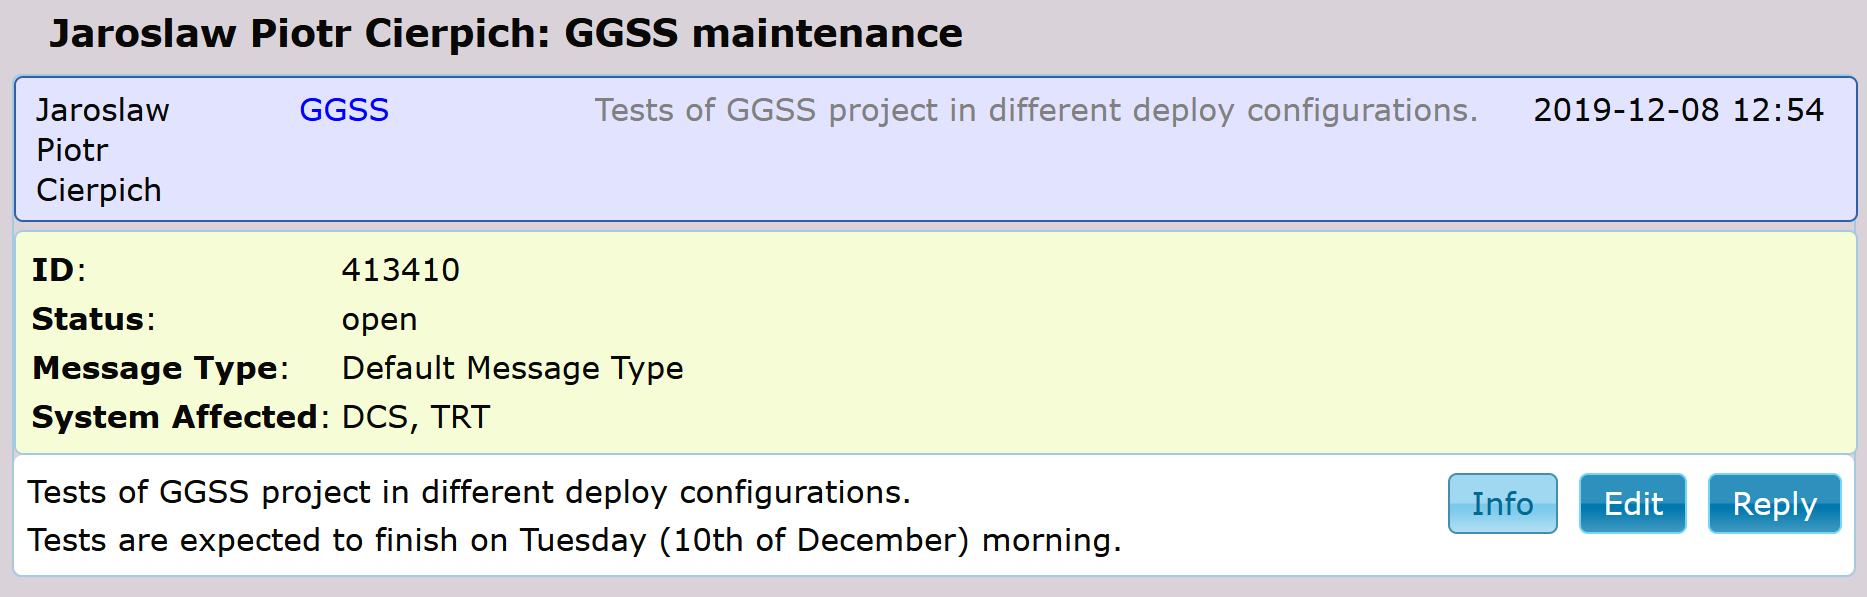
\includegraphics[width=\textwidth]{res/png/elisa}
\end{figure}

Pliki wykonywalne aplikacji \textit{ggssrunner} wygenerowane zostały za pomocą przygotowanego przez autorów środowiska CI/CD. Zostały one umieszczone na komputerze produkcyjnym. Kolejnym krokiem było zalogowanie się do panelu \textit{WinCC OA} służącego do monitorowania działania detektora ATLAS oraz wybranie panelu odpowiedzialnego za dostarczanie informacji o systemie GGSS. 

\begin{figure}[H]
\centering
\caption{Panel WinCC OA monitorujący działanie systemu GGSS}
\label{fig:ggss}
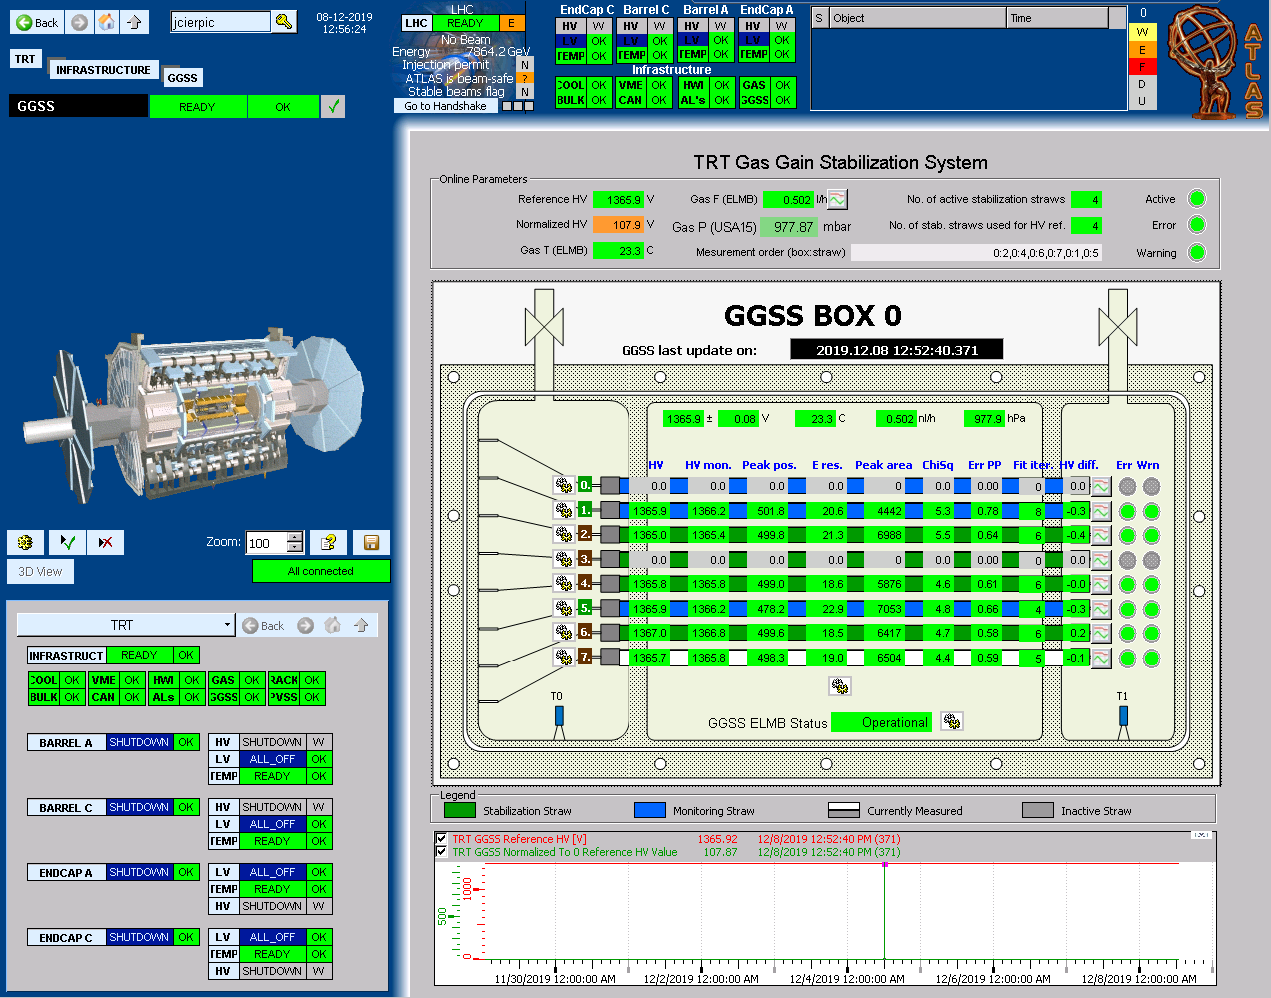
\includegraphics[width=\textwidth]{res/png/ggssStraw}
\end{figure}

Następnym etapem było przeprowadzenie procesu wyłączania systemu GGSS za pomocą przycisku \textit{Stop} znajdującego się na dedykowanym panelu konfiguracyjnym ukazanym na Rys. \ref{fig:ggsspanel}. 

\begin{figure}
\centering
\caption{Panel konfiguracyjny systemu GGSS podczas działania systemu}
\label{fig:ggsspanel}
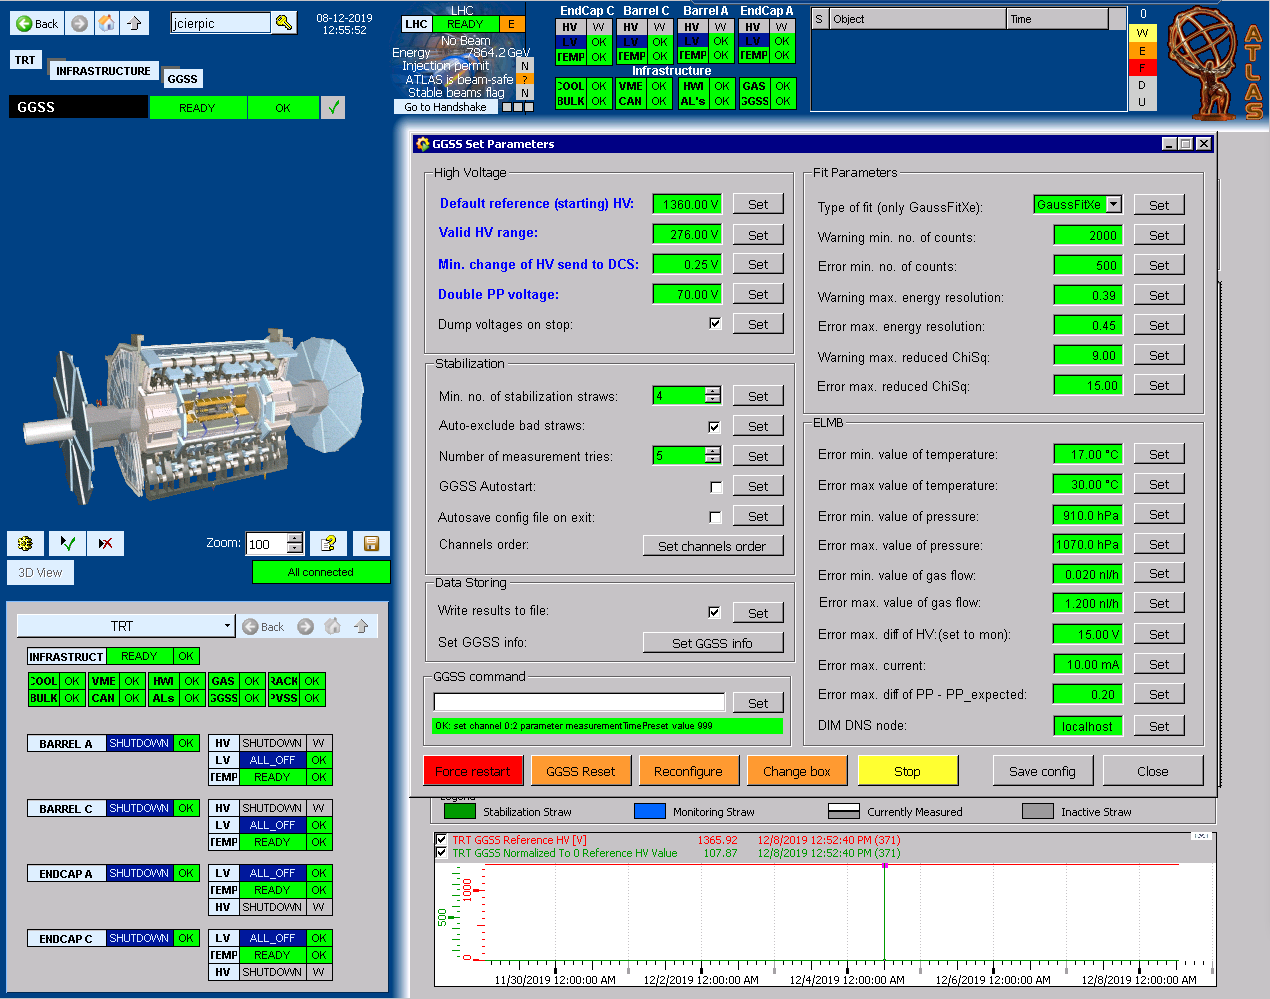
\includegraphics[width=\textwidth]{res/png/ggssConfig}
\end{figure}

Po wyłączeniu systemu należało również przerwać działanie poprzedniej wersji aplikacji \textit{ggssrunner} za pomocą skryptu \textit{ggss\_monitor.sh} (listing). Za pomocą tego skryptu został również potwierdzony stan aplikacji po wyłączeniu.

\textbf{tu kiedys bedzie listing jak Jarek nie wylaczy konsoli}


Po wykonaniu wyżej wymienionych czynności podmieniony został plik wykonywalny aplikacji \textit{ggssrunner} na przygotowany przez autorów. Zmiana została wykonana poprzez modyfikacje \textbf{dowiązania symbolicznego}. Następnie aplikacja uruchomiona została ponownie za pomocą skryptu \textit{ggss\_monitor.sh} (listing) oraz z poziomu panelu \textit{WinCC OA}. Stan panelu monitorującego system GGSS jest widoczny na Rys. \ref{fig:ggssafterstart}.

\begin{figure}
\centering
\caption{Panel WinCC OA monitorujący działanie systemu GGSS po ponownym uruchomieniu systemu (widoczny w lewym górnym rogu stan \textit{STARTING})}
\label{fig:ggssafterstart}
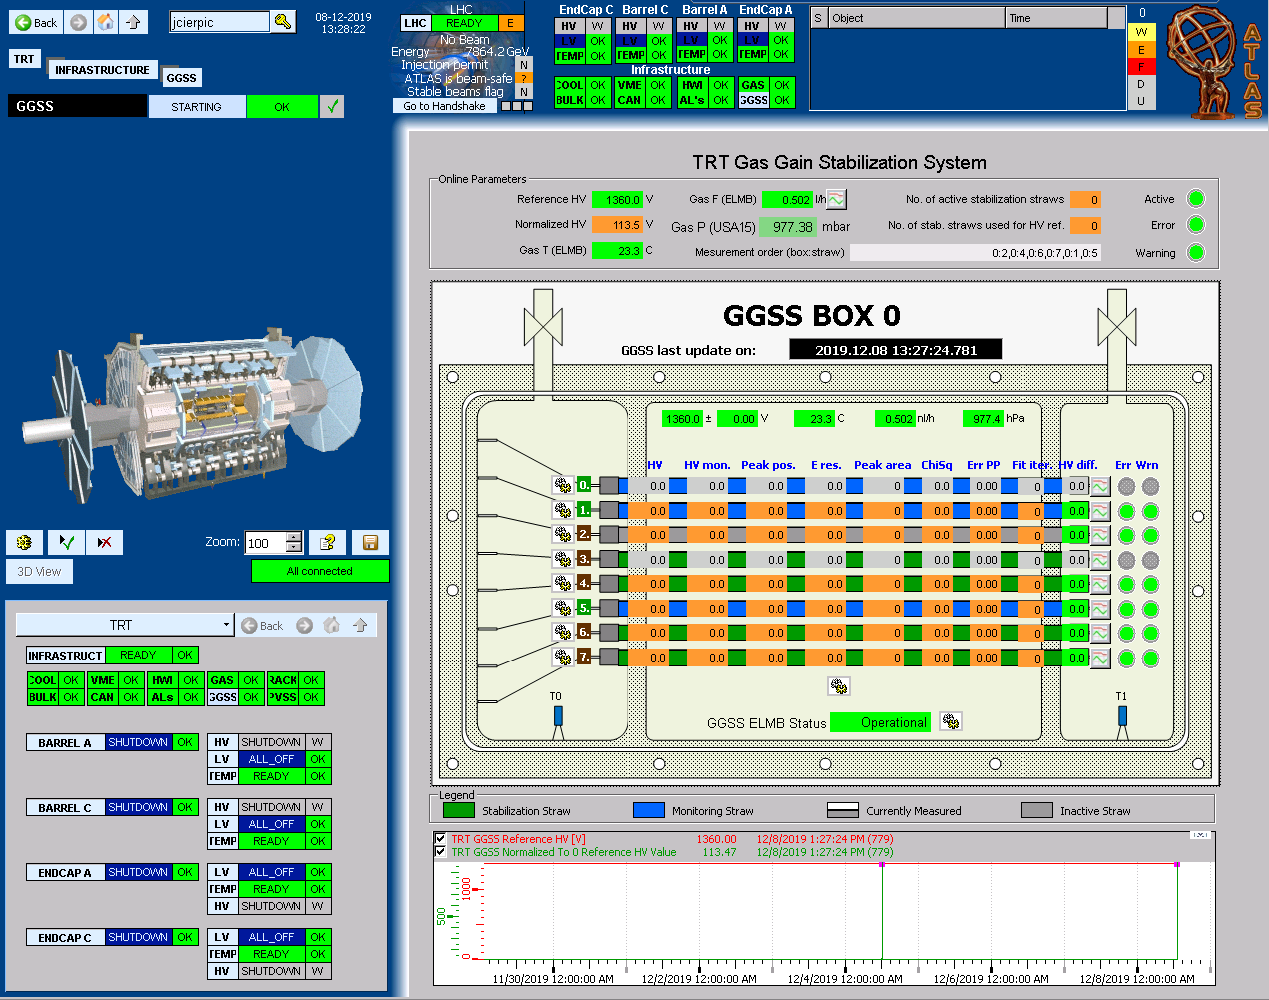
\includegraphics[width=\textwidth]{res/png/ggssPoStarcie}
\end{figure}

Dodatkowo użyty został skrypt pozwalający na monitorowanie zużycia zasobów pamięci przez aplikację (listing \ref{lst:ggssmem1}). Sposób użycia oraz fragment generowanego przez ten skrypt wyjścia przedstawia listing \ref{lst:ggssmem2}. 

\begin{lstlisting}[language=bash, caption={Skrypt \textit{check\_mem\_ggssrunner.sh} służacy do monitorowania pamięci używanej przez aplikację \textit{ggssrunner}}, label={lst:ggssmem1}]
#!/bin/bash
while true
do
    ps afux | egrep " ./ggssrunner" | awk -v date="$(date +"%Y.%m.%d %H:%M:%S")" '{print date, $5}'
    sleep 1m
done
\end{lstlisting}


\begin{lstlisting}[language=bash, caption={Wywołanie oraz fragment wyjścia skryptu \textit{check\_mem\_ggssrunner.sh} służacego do monitorowania pamięci używanej przez aplikację \textit{ggssrunner}}, label={lst:ggssmem2}]
user@host:~$ ./check_mem_ggssrunner.sh
2019.12.08 15:15:26 638800
2019.12.08 15:16:26 638800
2019.12.08 15:17:26 638800
2019.12.08 15:18:26 638800
2019.12.08 15:19:26 638800
2019.12.08 15:20:27 638800
2019.12.08 15:21:27 638800
2019.12.08 15:22:27 638800
\end{lstlisting}

\section{Wyniki testu}
Test każdej z czterech przygotowanych konfiguracji trwał \textbf{ponad 6 godzin}. Tabela \ref{tab:wyniki} przedstawia rezultaty.

\begin{table}[H]
\begin{tabular}{|c|c|c|c|}
\hline
\rowcolor[HTML]{ECF4FF} 
\textbf{\begin{tabular}[c]{@{}c@{}}Konfiguracja \\ (debug/release)\end{tabular}} & \textbf{\begin{tabular}[c]{@{}c@{}}Sposób linkowania \\ biblioteki Boost\end{tabular}} & \textbf{Wygenerowane błędy} & \textbf{Zużycie pamięci} \\ \hline
debug                                                                            & statyczne                                                                              &                             &                          \\ \hline
release                                                                          & statyczne                                                                              &                             &                          \\ \hline
debug                                                                            & dynamiczne                                                                             &                             &                          \\ \hline
release                                                                          & dynamiczne                                                                             &                             &                          \\ \hline
\end{tabular}
\caption{Wyniki testów aplikacji \textit{ggssrunner}}
\label{tab:wyniki}
\end{table}

\textbf{jakos to skomentowac jak beda wszystkie}